% Chapter 9

\chapter[Implementation]{Implementation} % Main chapter title

\label{Chapter9} % For referencing the chapter elsewhere, use \ref{Chapter9} 

%----------------------------------------------------------------------------------------

This section gives details of the implementation phase of the project, including descriptions of how parts of the system function, information regarding the development process and explanations for some of the key decisions made regarding the implementation.

\section{Overview}
The system was implemented closely following the design laid out in chapter \ref{Chapter8}, and comprises two parts; the main computer software application (referred to henceforth as `the application') and a collection of software routines designed to be included within the code on the robots, which form an `application programming interface' (API) . This API (referred to as the 'robot side code' or 'robot side API') provides the developer with functions to send data from the robot back to the application, and contains routines for handling the networking requirements to achieve this, and for correctly formatting the data. Details of this robot side API are provided in section \ref{RobotSide}. Both parts of the system implementation are fully independent. The application can be run on its own and receive data from any source, provided that this data correctly follows the format outlined in section \ref{DataTransferFormat}. The robot side code could be used to send data to another host, provided that the robot uses the correct target IP address and port number, and again provided that the host can correctly interpret the data format. The application is the much larger of the two system parts, and therefore will be the focus of the majority of this implementation chapter.

Figure \ref{fig:UI} shows the user interface for the application as it is seen at start-up. This can be compared to figures \ref{fig:UILayout} and \ref{fig:UIExample} to see the relationship to the user interface design. The key features of the application can be seen in this image. The visualiser component shows the video feed, augmented with information about the three visible robots, including position, direction, ID number, and the selected robot's name and current state. The robot list panel is visible on the right hand side, showing the IDs and names of the known robots, and which of them is currently selected. Finally the data panel can be seen at the bottom of the application, currently set to the overview tab, providing summary information about the selected robot. More detailed information about the implementation of the UI itself can be found in section \ref{UserInterfaceImplementation}.

\begin{figure}
	\centering
	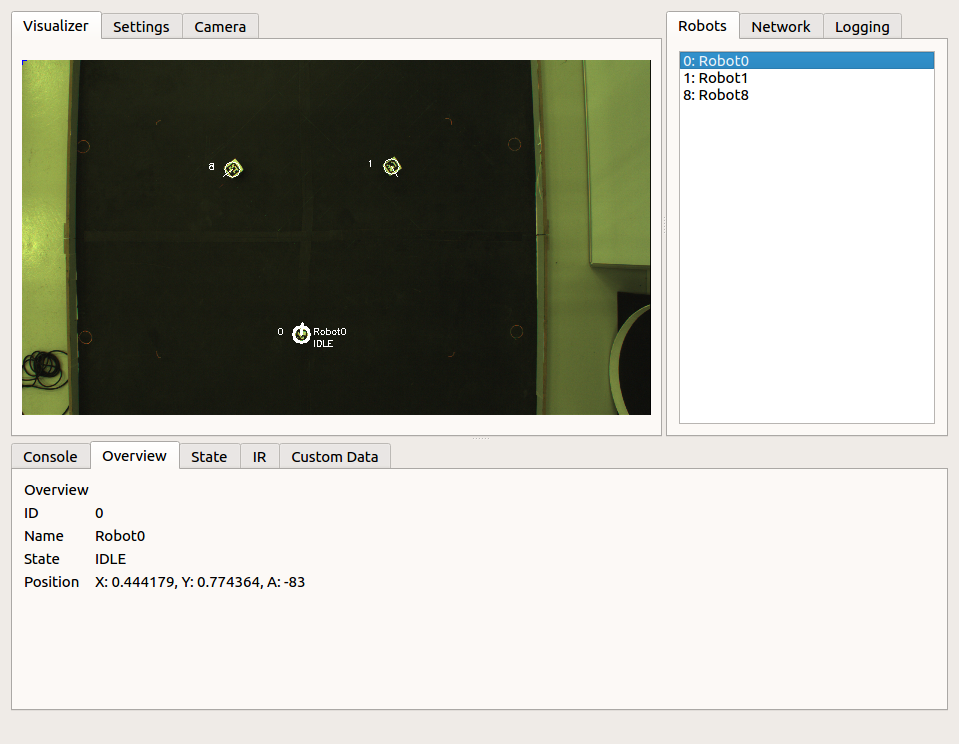
\includegraphics[scale=0.4]{Figures/ApplicationScreenshotOverview.png}
	\decoRule
	\caption[Application User Interface]{The user interface for the application.}
	\label{fig:UI}
\end{figure}

\section{Application Framework Selection} \label{ApplicationFrameworkSelection}
Developing computer software applications often involves implementing a large amount of the same low level functionality, regardless of the application. This includes low level back end functionality such as event management and dissemination, standard constructs such as timers and threads, as well as standard user interface elements such as windows, menus, panels, lists, tables, buttons and many more. It is clear that these functionalities are independent of the purpose of the application being developed, and implementing them from scratch for each new application would require a huge amount of time, and therefore be extraordinarily inefficient. For this reason the vast majority of modern software is created using some kind of application programming framework.

The purpose of these frameworks is to provide common, low level application functionality in the form of an API, which the developer can then leverage to develop their specific application. The API will usually include a number of classes to define the common UI elements, and a hierarchical tree- or node-based structure the developer can populate with these elements to create their desired UI. Most computer applications are event driven; when the user provides some kind of input such as a click or a key press an event is generated, and this event will be different depending on which UI component the user was interacting with. This event then needs to be disseminated through the application in order to trigger the correct functionality. Most application programming interfaces will handle the generation and dissemination of these events, allowing the developer to `\textit{register}' code to be executed in response to specific events. The developer can therefore simply focus on implementing the functionality that is unique to their application.

Most modern application frameworks contain a wide variety of features in addition to those responsible for the UI and event management. These can include everything from low level components such as timers, input/output (I/O) interfaces, and networking components, to higher level multimedia handlers such as video and audio players, and rich HTML viewers. Frameworks also might include classes for creating data models which can be easily mapped to more complex user interface elements such as responsive tables.

Selecting an appropriate framework to use as the basis for this application was one of the first steps in the implementation process. All of the available frameworks have different benefits and limitations, and target a variety of different platforms, operating systems, and languages. During the design phase it was determined that the application should be implemented in C++, for reasons discussed in section \ref{SoftwareArchitectureDesign}. This therefore eliminated a number of frameworks, such as the Oracle Application Development Framework which is specific to the Java language, and Microsoft's .NET framework, which is C\# specific. The application also needed to run on the server connected to the tracking camera, which runs a Linux operating system. This therefore ruled out any Windows specific frameworks, including one of the most widely used C++ frameworks, the Microsoft Foundation Class Library (MFC).

\subsection{The \textit{Qt} Framework}
It was determined that the `\textit{Qt}' application framework was the most suitable for this application, as it provides support for cross-platform compilation, including Linux, and is implemented natively in C++. A number of factors, in addition to the target platform and language, influenced this decision. The framework is widely used, and therefore has a well-tested, refined, and mature API, with a good body of documentation available. It provides a comprehensive library of classes for a range of common application functionalities, including GUI front-end and low level back-end components. The framework also includes built-in support for multi-threading, and a structured `\textit{Signals and Slots}' system for sending and receiving event notifications, and moving data between components and across threads. For an application such as this, with a number of external data sources in addition to the user input, and a multi-threaded design, this was determined to be a highly beneficial feature which could reduce development complexity significantly. Furthermore previous experience with Qt outside of this project had been positive, and meant a smaller learning curve would be necessary to begin developing the application. For non-commercial projects Qt is available free of charge, making it a good fit for an academic project.

The following primary features of the Qt application framework were used within this project:

\begin{itemize}
 \item Standard GUI components and layout management classes used to create the majority of the user interface.
 \item Event management system to handle user input events.
 \item `\textit{QTimer}' component to implement timers and recurring events, such as camera polling.
 \item `\textit{QThread}' API to partition the application components into threads.
 \item `\textit{Signals and Slots}' system for inter-component and inter-thread signalling and data transfer.
 \item `\textit{QPainter}' component for rendering custom user interface elements.
\end{itemize}

%----------------------------------------------------------------------------------------

\section{Application Structure} \label{ApplicationStructure}
The application has been implemented closely following the software architecture design outlined in section \ref{SoftwareArchitectureDesign}. Figure \ref{fig:ApplicationStructure} shows the structure of the application at a class level following implementation, with the arrows showing the flow of data. All of the main classes are displayed, with some of the minor classes omitted for clarity. Comparing this with the software architecture design we can see that the \textit{MainWindow} class encapsulates the functionality of the application controller block, forming the core of the application and routing data between the other components. This class is instantiated when the application begins, and performs all of the set up operations. This involves constructing and initialising the user interface based on the layout defined in \textit{mainwindow.ui}, creating instances of the main components, connecting the related signals and slots of each component, and moving the components to their appropriate threads. 

The output signals generated by the \textit{DataThread} class when new robot data arrives, and the \textit{CameraController} class when new tracking data is available, are routed to the \textit{DataModel} class's \textit{new data} input slot. Similarly the signal generated by the \textit{CameraController} class when a new video frame has been acquired is routed to the \textit{Visualiser} class's \textit{image data} slot. In figure \ref{fig:ApplicationStructure}, these signal/slot connections are represented by dotted arrows. Singleton instances for the \textit{Settings} and \textit{Log} classes are also created during initialisation, which allow the settings and logging functions to be accessed from anywhere in the application. 

Following initialisation, whilst the application is running, the \textit{MainWindow} class is responsible for handling user input events sent from the UI, modifying the other classes as necessary depending on the input event received. Finally, when the application is closed, the \textit{MainWindow} class is responsible for tearing down the other components. This involves stopping any active timers, stopping the various threads, and releasing all allocated memory.

\begin{figure}
	\centering
	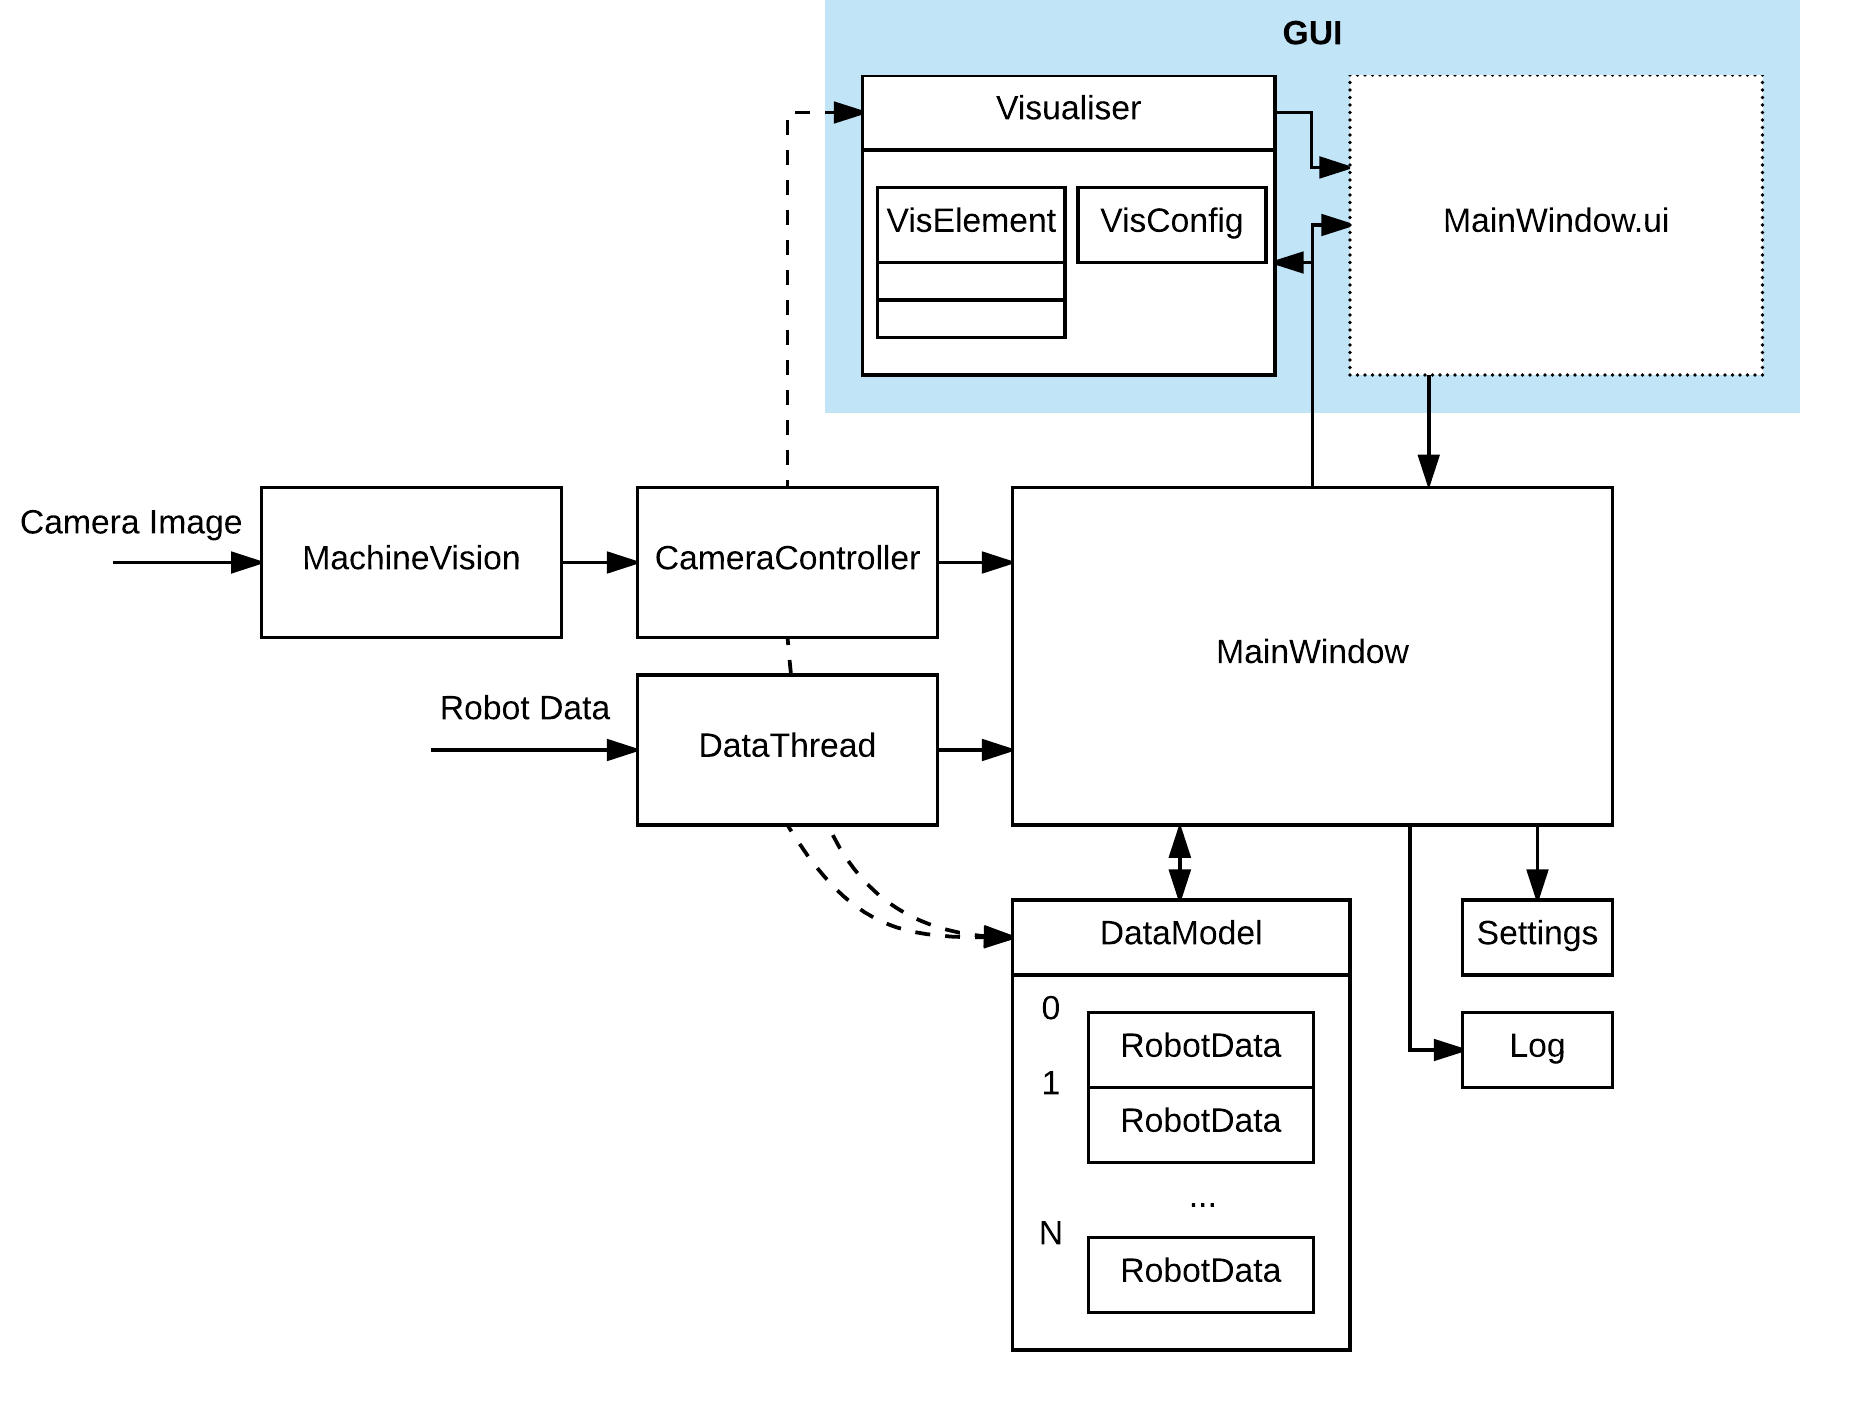
\includegraphics[scale=0.8]{Figures/ApplicationStructure.png}
	\decoRule
	\caption[Application Structure]{The structure of the classes within the application. Arrows represent the data path.}
	\label{fig:ApplicationStructure}
\end{figure}

The GUI portion of the software architecture design is encapsulated into the UI description file \textit{mainwindow.ui}, which then connects back to the \textit{MainWindow} class through Qt's UI event management system. Section \ref{UserInterfaceImplementation} provides details of the user interface implementation. The visualiser portion of the GUI is encapsulated into the \textit{Visualiser} class, which handles generating the graphical overlays, applying them to the latest video image, and displaying the resulting augmented video image. Generating the overlays involves a number of smaller classes, as shown in figure \ref{fig:ApplicationStructure}. Section \ref{VisualiserImplementation} provides more detail about the implementation of the visualiser class and its sub-classes. The camera controller and tracking code components are encapsulated in the \textit{CameraController} and \textit{MachineVision} classes respectively, discussed further in section \ref{VideoFeedAndTrackingSystem}, and the network controller component is implemented in the \textit{DataThread} class, which is discussed in section \ref{Networking}. Finally the data model component is implemented in the \textit{DataModel} class, making use of the smaller \textit{RobotData} class as per the design in section \ref{DataModelDesign}. This implementation is discussed in section \ref{DataModel}.

%----------------------------------------------------------------------------------------

\section{Source Code}
The system source code is implemented in two groups of files; a collection of C++ source and header files which make up the main application, and a smaller collection of C++ source and header files which handle the robot-side portion of the system. In addition to its source files, the main application also relies on a number of other files which are used by the Qt system to define the user interface layout, and manage the build process. A full list of all source code files is given in appendix \ref{AppendixSourceCodeFiles}. Table \ref{tab:CodeFiles} details the names and purposes of all files within the main application. Table \ref{tab:RobotCodeFiles} details the files that make up the robot side API.

%----------------------------------------------------------------------------------------

\section{Data Model} \label{DataModel}
The data model forms a core element of the back end of the application. For each robot being tracked by the system, the data model is required to store the information related to that robot. This is done in a structured manner, such that other parts of the application can query specific data within the model easily. The contents of the data model are updated whenever new data arrives, and are consulted when rendering the user interface. Section \ref{DataModelDesign} describes the design of the data model and its hierarchical structure. The implementation follows this design closely, with the \textit{DataModel} class contained in \textit{datamodel.cpp / .h} encapsulating the top level data model container, and the individual robot data object encapsulated in the \textit{RobotData} class in \textit{robotdata.cpp / .h}.

The \textit{DataModel} class uses a standard C++ `\textit{vector}' container to maintain a list of \textit{RobotData} objects. Each of these \textit{RobotData} objects describes one robot that is currently known to the system. The list is ordered based on the robots' IDs, and is sorted after each new insertion. The vector container was chosen as it does not require a fixed size, and can be sorted and iterated efficiently. The \textit{DataModel} class provides convenience functions for data retrieval functionality, such as retrieving the data object for a given robot based on ID number. It also provides a function for entering new data into the model, which inherits the properties of a `\textit{slot}' within the Qt framework, allowing it to be called from other threads. Each new data packet received from the network is routed to this slot, as well as position data obtained from the tracking system. All data is supplied in the form of a string in one of the packet formats described in section \ref{DataTransferFormat}. Code within the data model class then handles interpreting the string, determining its purpose and source robot, separating out the data content, and updating the relevant robot within the model. Whenever data arrives from a previously unknown robot, this code handles creating a new \textit{RobotData} object, and adding it to the list.

The \textit{RobotData} class encapsulates the data for a single robot. This involves storing a number of different data points, in a variety of different formats. The class then acts as a relatively simple container for this data, providing functions for retrieving and changing values. Table \ref{tab:RobotDataContents} outlines the data points contained within the class.

\begin{longtable}{ l l p{8cm} }
\caption[Robot Data Contents]{The contents of the \textit{RobotData} class.}\\
 \hline
 Data Point & Type & Description\\
 \hline\\
 Robot ID & Integer & The numerical ID of the robot, used by the tracking system and when transmitting data.\\
 Robot Name & String & The name associated with this robot. Set by the user when programming the robot, and reported in watchdog packets. \\
 State & String & The current state of the robot. \\
 Known States & List of Strings & A list of all states the robot has previously reported. \\
 Position & 2D Vector & The current position of the robot expressed as a proportional coordinate vector. \\
 Angle & Integer & The current angle of the robot in degrees. \\
 Colour & OpenCV Scalar & The colour used for this robot in the visualiser, if colours are enabled, expressed as an OpenCV Scalar struct in BGR format. \\
 IR Data & Array of Integers & The most recent IR sensor readings for this robot. One value per sensor. \\
 Background IR Data & Array of Integers & The most recent background IR sensor readings. One value per sensor. \\
 Custom Data & Key Value Map & All custom user data. Stored as a map of key/value pairs. \\
 \bottomrule\\
 \label{tab:RobotDataContents}
\end{longtable}

In addition to this data, the class also maintains a list of recent state transitions, and a short term history of the robot's position. The state transition list uses a custom structure to store the state before the transition, the state after the transition, and the time the transition occurred. A fixed size array of these custom structures is maintained and updated each time a state transition occurs, acting as a first-in first-out (FIFO) queue. The position history is stored in a similar fashion, using a fixed size array of coordinate pairs, which is updated every Nth position update. This interval can be configured by the user, with a lower interval giving a higher resolution but a shorter history, and vice versa for a higher interval. Functions are provided to retrieve data from these queues when needed.

%----------------------------------------------------------------------------------------

\section{Video Feed and Tracking System} \label{VideoFeedAndTrackingSystem}
Functionality for acquiring images from the machine vision camera, and running the ArUco tag tracking algorithm, is encapsulated in the \textit{CameraController} and \textit{MachineVision} classes, which are implemented in \textit{cameracontroller.cpp / .h} and \textit{machinevision.cpp / .h} respectively. Video is retrieved from the camera one frame at a time, and can therefore be thought of as a sequence of discreet images. A call to the camera driver to obtain the next image might block execution whilst it waits for the image to become available. Hence in order to maximise application performance and ensure responsiveness these classes are run on a separate thread dedicated to camera functionality. 

The \textit{CameraController} class handles the higher level operations such as running a timer to periodically poll for the next image, supplying the correct dimensions for the image, and converting the image and tracking data into formats which can be passed back to the main thread and used in the UI and data model respectively. The application threading is handled through the use of the Qt framework's \textit{QThread} API, and communication between threads utilises the framework's `\textit{signals} and \textit{slots}' feature, which allows components on different threads to send and receive data in a managed, thread-safe manner. The \textit{CameraController} class therefore utilises two signals; one for emitting the camera image data, and another for emitting the robot position data. At initialisation time the application's core class, \textit{MainWindow}, connects these signals to matching slots within the \textit{Visualiser} and \textit{DataModel} classes respectively.

The \textit{MachineVision} class handles the lower level operations related to the camera and the tracking system, including setting up the camera driver, retrieving and resizing individual images from the camera, and running the ArUco tag detection algorithm. The ArUco software is implemented as an additional component of the OpenCV image processing library (discussed below), and provides a function to run the tag detection algorithm on a given image, for a given dictionary of tags. For each tag detected in the image that matches one in the chosen dictionary, the ArUco algorithm returns the pixel coordinates of the four corners of the tag. The \textit{MachineVision} class includes code to average these four coordinates, acquiring a central pixel coordinate, which is then converted to a 'proportional' coordinate; two numbers between 0 and 1 which represent the horizontal and vertical components of the position as a proportion of the full height and width of the image respectively. This ensures that a robot's position can still be correctly displayed after the image has been resized, without having to maintain information related to the resizing operation. The angle the robot is facing is also calculated. This is done by first calculating the coordinate of the fourth corner in a coordinate system where the third corner is positioned at the origin, and then applying an arctangent function to this coordinate to obtain the angle. This angle is then converted to degrees and stored as an integer in order to reduce complexity, as a precision greater than one degree was not deemed necessary.

%----------------------------------------------------------------------------------------

\subsection{The \textit{OpenCV} Image Processing Library}
A number of the components within the application are required to manipulate image data. The image data acquired from the tracking camera by the \textit{CameraController} and \textit{MachineVision} classes must be stored in a format that can be processed by the ArUco tag detection algorithm. This image data must then be passed to the \textit{Visualiser} class, which renders the graphical overlays on top. Selecting a suitable image processing library was one of the early steps in the implementation process. The ArUco tag detection algorithm is implemented as an extension to the \textit{OpenCV} image processing library, so this seemed to be obvious choice. However the Qt framework supports its own image data format and drawing classes, so the image could be converted to this format once the tracking data had been extracted. OpenCV is a widely used, feature-rich, powerful image processing library, and ultimately it was decided that all image manipulation should make use of it where possible. It was hoped that this would improve maintainability in the future, as OpenCV is more widely used, and also improve portability. If the code was ever to be ported away from the Qt framework, image processing functionality implemented using OpenCV would require less change.

%----------------------------------------------------------------------------------------

\section{Networking} \label{Networking}
A key element of the system is the wireless retrieval of information from the robots. This required the implementation of networking functionality within both the application and the robot side API. As mentioned previously the Linux extension boards on the e-puck robots feature a WiFi adapter, so WiFi was selected as the target wireless networking technology to implement this functionality with. The next step was to look at the networking requirements in more detail, and decide on which transport layer protocol to use.

The requirements for the networking portion of the system were relatively simple, and can be summarised as follows:

\begin{enumerate}
	\item Must utilise a WiFi network.
	\item Must allow a large number of sources to transmit data to a single host.
	\item Must allow for frequent transmission of small packets of data.
\end{enumerate}

WiFi networks utilise the standard Internet Protocol (IP) \cite{TCPIP} network layer protocol. There are two commonly supported transport layer protocols which run on top of IP, the Transmission Control Protocol (TCP) and the User Datagram Protocol (UDP). TCP is a managed and delivery-error checked protocol, and therefore guarantees that packets will be transmitted in the correct order, with lost packets being retransmitted. This adds overheads such as acknowledgements to the protocol, and requires an established 'connection' in order to function correctly. TCP also operates a queueing system, whereby packets for transmission are sometimes held until a number of them are ready, and can therefore be grouped together and sent. 

UDP \cite{UDP}, by contrast, does not error check the delivery of packets, making no guarantees that a packet will be received, or that packets will be received in the correct order, removing the need for an established connection and reducing the overheads involved. Packets can therefore be sent from any application to any target IP address and port on the network, without first establishing a connection with another application. Packets are also sent immediately, with no queueing system in place. It was determined that UDP would be the most suitable for this system, for a number of reasons. The connection requirements of TCP would require the application to form a connection with each robot prior to transmitting data, which would add unnecessary complexity. Using UDP also ensured that the packets were transmitted immediately, reducing the potential for latency in the system. The lack of delivery checking was not considered an issue, as the robots would be transmitting updates frequently enough that a single lost packet would not cause a significant issue.

The networking functionalities of the application are encapsulated in the \textit{DataThread} class, found in \textit{datathread.cpp / .h}. This class is run on a dedicated thread to ensure that potentially blocking operations do not impact application performance. The class contains routines for dealing with the low level network requirements, such as establishing a socket through which to receive data packets from the robots, and continually listening on this socket for new data. Figure \ref{fig:NetworkingFlow} shows the operation of the \textit{DataThread} class as a flow diagram. The `\textit{Packet Listening Started}' signal, highlighted in green, is generated when the user presses the `\textit{Start Listening}' interface button in the networking tab. All socket operations are implemented using structures and definitions from the standard C++ networking libraries. 

Data received from the robots is passed to the main application thread through a Qt signal, using the Qt signals and slots interface mentioned previously. The main application class, \textit{MainWindow}, connects this signal to the appropriate slot in the \textit{DataModel} class at initialisation time. The application side networking can be configured by the user in the \textit{network} tab of the right-hand panel of the user interface. Here the user is able to enter a desired port number on which to receive data, and can start and stop the application listening for packets on this port by pressing the `\textit{start/stop listening}' button.

\begin{figure}
	\centering
	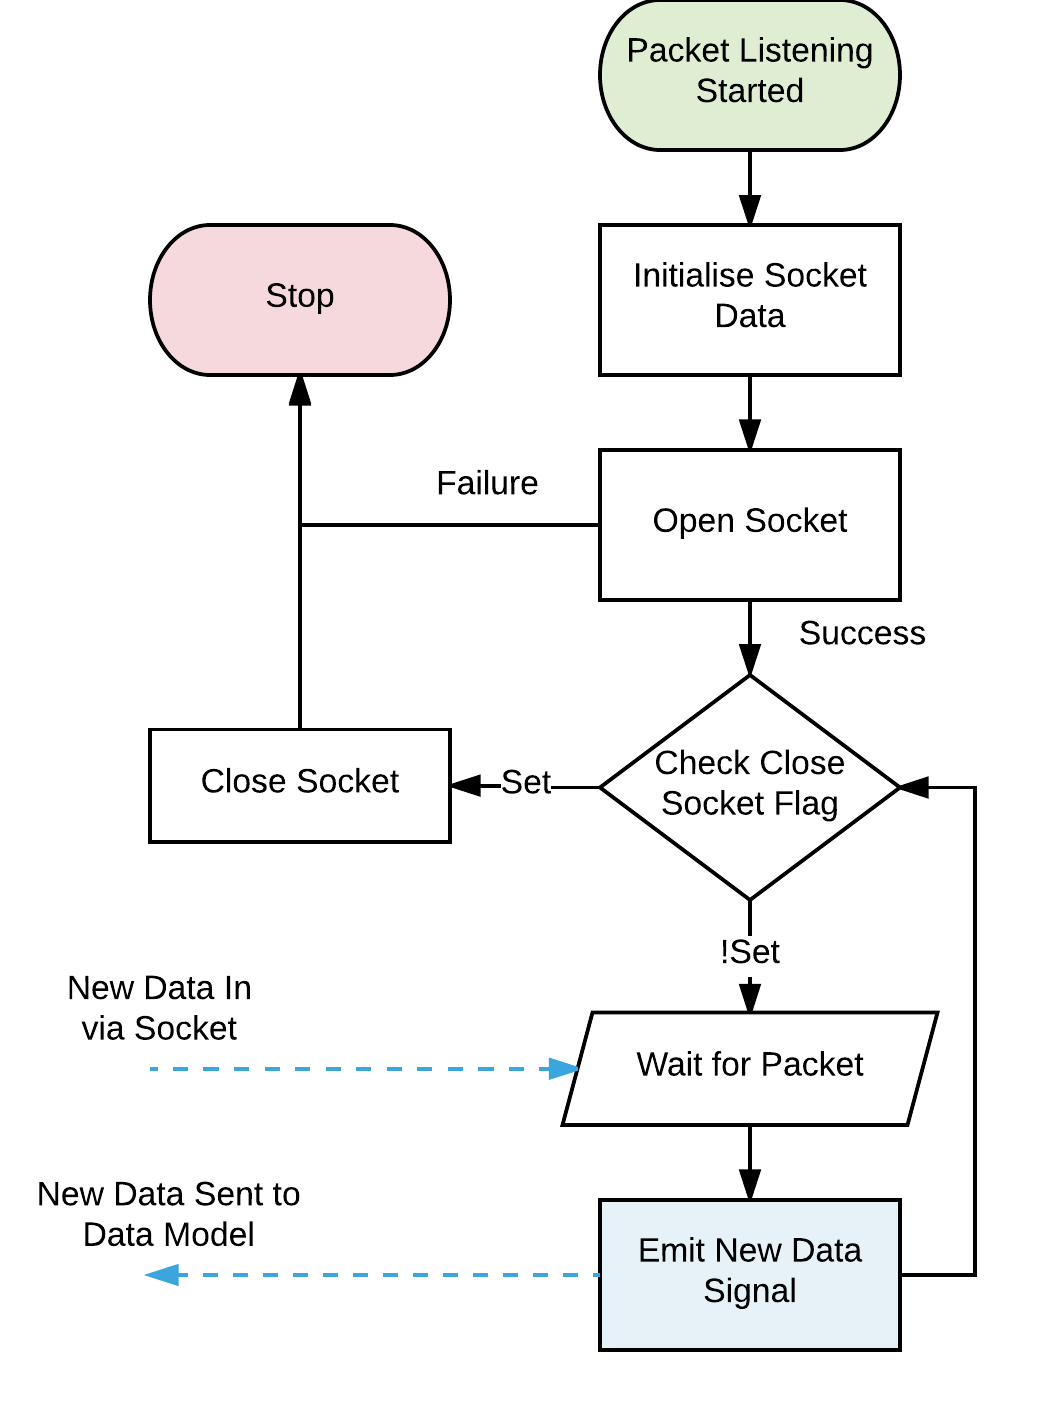
\includegraphics[scale=1]{Figures/NetworkingFlow.png}
	\decoRule
	\caption[Networking Code Flow Diagram]{A flow diagram showing the sequence of operations carried out by the \textit{DataThread} networking class.}
	\label{fig:NetworkingFlow}
\end{figure}

For the robot side API, the networking functionality is implemented in a similar way. The initialisation function establishes a target socket based on a supplied IP address and port. This should match the IP address of the computer or server running the main application, and the port chosen by the user within the main application. When any of the functions for sending specific data packets are called, the data is sent to this target socket as a UDP packet. Section \ref{DataTransferFormat} discusses the format of the data within these packets. All socket operations are once again implemented using the standard C++ networking libraries to increase portability.

%----------------------------------------------------------------------------------------

\section{Data Transfer Format} \label{DataTransferFormat}
In order for the application to interpret and use data received from the robots, a common format for exchanging this data needed to be defined. Both sides of the communication link then need to use this format correctly when constructing and de-constructing packets. A number of different options were considered for achieving this, ranging from super-lightweight custom packet formats using the minimum number of bytes, to established existing solutions such as the JSON data interchange standard. The primary concerns when making this decision were a desire to minimise any overheads in terms of extra code needed on the robot side, as the robots have limited memory, and to ensure the format remained as simple as possible so that future extensions to the system, such as implementations for other robots, could be programmed with relative ease. The size of packets was also a concern, as minimising network traffic where possible would benefit the system if used with a large number of robots.

It was ultimately decided not to use JSON, to avoid the need for any additional code libraries to be stored in the robot's memory, and to instead use a custom, simple, string-based packet format. All data to be transmitted from the robot to the application is therefore converted to a string which is then transmitted in the data packet. As well as containing the data, the string must identify the robot and describe the type of data within. The format for these strings is defined as three sections separated by space characters. The first section contains the numerical ID of the robot sending the packet. The second contains a number identifying the type of data contained in the packet. The last section contains the packet data, and has a variable format, depending on the packet's type. Figure \ref{fig:DataFormat} gives a visual representation of this format. Table \ref{tab:DataFormat} describes the purpose of each packet type, and describes the format of the `packet data' section for each. An example of each packet type is given, using the arbitrary robot ID of 6.

\vspace{2cm}

\begin{figure}[h]
 \centering
 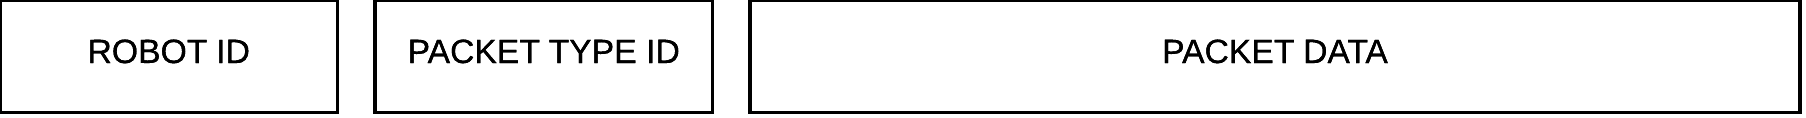
\includegraphics[scale=0.3]{Figures/DataFormat.png}
 \decoRule
 \caption[Data Format]{The general format for each data packet.}
 \label{fig:DataFormat}
\end{figure}

\clearpage
\begin{longtable}{ l p{12cm} }
\caption[Data Format]{The format of the data section and the purpose of each packet type.}\\
 \hline
 \multicolumn{2}{p{12cm}}{\textbf{Watchdog Packet}}\\
 \hline
 Type ID & 0 \\
 Format & [ROBOT NAME]\\
 Purpose & Sent periodically to inform the application that the robot is still active. Also contains the robot's name, as should be displayed in the application.\\
 Example & ``6 0 Robot\_6''\\
 
 \hline
 \multicolumn{2}{p{12cm}}{\textbf{State}}\\
 \hline
 Type ID & 1 \\
 Format & [CURRENT STATE]\\
 Purpose & Informs the application of the robot's current state.\\
 Example & ``6 1 IDLE''\\
 
 \hline
 \multicolumn{2}{p{12cm}}{\textbf{Position}}\\
 \hline
 Type ID & 2 \\
 Format & [X POSITION] \_ [Y POSITION] \_ [ANGLE]\\
 Purpose & Provides the application with a robot's position and orientation. This data is not sent by the robot, but instead comes from the tracking code.\\
 Example & ``6 2 0.23 0.682 110''\\
 
 \hline
 \multicolumn{2}{p{12cm}}{\textbf{IR}}\\
 \hline
 Type ID & 3 \\
 Format & [SENSOR 1 DATA] \_ [SENSOR 2 DATA] \_ ... [SENSOR N DATA] \\
 Purpose & Contains a robot's infra-red sensor readings. Each sensor value is separated by a space, and the packet can contain as many values as the robot has IR sensors. \\
 Example & ``6 3 101 93 115 112 103 98 365 2850''\\
 
 \hline
 \multicolumn{2}{p{12cm}}{\textbf{Background IR}}\\
 \hline
 Type ID & 4 \\
 Format & [SENSOR 1 DATA] \_ [SENSOR 2 DATA] \_ ... [SENSOR N DATA] \\
 Purpose & Contains a robot's background infra-red sensor readings. Formatted the same as the standard IR data packet.\\
 Example & ``6 4 95 87 99 110 89 98 103 82''\\
 
 \hline
 \multicolumn{2}{p{12cm}}{\textbf{Message}}\\
 \hline
 Type ID & 5 \\
 Format & [MESSAGE STRING]\\
 Purpose & This packet allows any general message to be sent from the robot to the application, and will be displayed in the application console and recorded in the logs. \\
 Example & ``6 5 Robot entering hibernation mode''\\
 
 \hline
 \multicolumn{2}{p{12cm}}{\textbf{Custom Data}}\\
 \hline
 Type ID & 6 \\
 Format & [KEY] \_ [VALUE]\\
 Purpose & Contains a piece of custom user data, in the form of a key value pair. \\
 Example & ``6 6 DebugCounter 540''\\
 \bottomrule
	
 \label{tab:DataFormat}
\end{longtable}

\subsection{Constraints}
For a number of the packet types constraints are placed on the input data, both in terms of format and in terms of the range of valid values. The space character is used as a delimiter to separate portions of the packet, hence in all cases except the message packet a space character cannot appear in the middle of any of the data. This means that robot names and states cannot include spaces, nor can custom data keys or values. The message packet type is an exception, and will treat any characters following the second space, which marks the end of the header data, as a single string. This string then forms the message content. 

For the watchdog, state, position and custom data packet types, the correct number of space-separated data portions must be included, or the string is invalid. This means one, one, three and two data portions respectively. In the case of the IR data a minimum of one data portion must be included, but there is no upper limit. Any portions above the number of supported sensors will be ignored. The IR data values must be positive integers in the range of 0 to 4095. Values outside of this range will be clamped to the closest value that satisfies this requirement. Floating point values will cause the packet to be marked as invalid and ignored. The numerical data in the position packet must be two floating point values (X and Y position), followed by one integer value (angle). A floating point value can be interpreted from an integer (the decimal point is therefore not necessary), however the integer angle value cannot be interpreted from a floating point data portion, and this will cause the packet to be marked as invalid and ignored by the application. 

%----------------------------------------------------------------------------------------

\section{User Interface} \label{UserInterfaceImplementation}
In order to implement the user interface the designs shown in section \ref{UserInterfaceDesign} had to be realised using the UI component classes provided by the Qt application framework. The `\textit{QtCreator}' tool was used to arrange all the basic elements of the UI, and generate an XML-based descriptor file (\textit{mainwindow.ui}) which describes this layout. When the application is initialised this file is parsed and used to populate the user interface. Events generated by the interface are linked to functions within the \textit{MainWindow} class using the signals and slots system. Code was then implemented within each of these functions to execute the correct actions based on the input received.

\begin{figure}
 \centering
 \makebox[\textwidth][c]{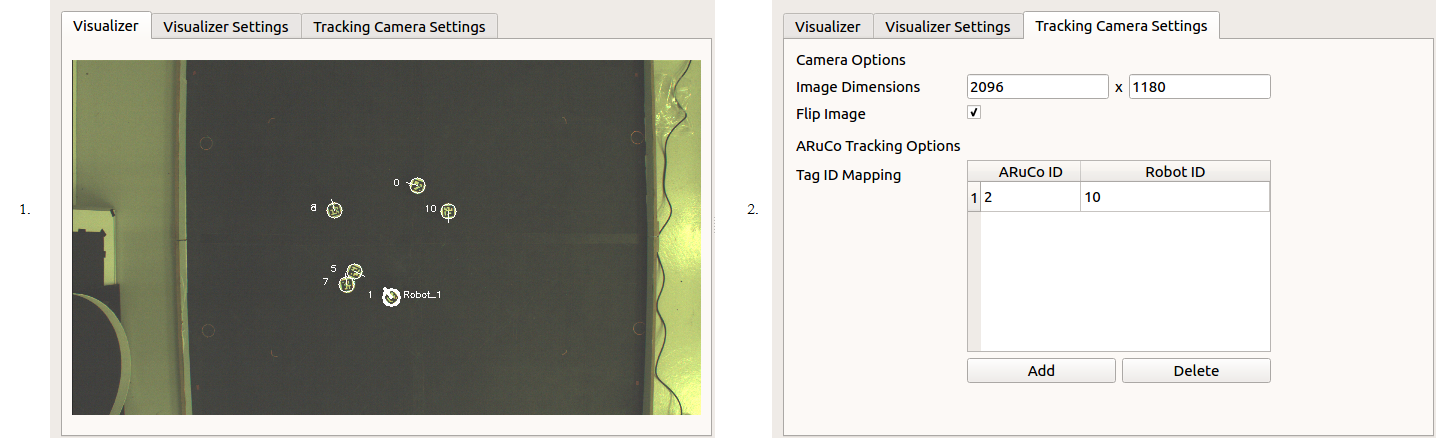
\includegraphics[width=1.3\textwidth]{Figures/VisualiserPanel.png}}
 \decoRule
 \caption[Visualiser Panel]{The visualiser panel, with two of the different tabs shown.}
 \label{fig:VisualiserPanel}
\end{figure}

The user interface was implemented following the three panel layout outlined during the design phase. The panels are divided by splitters which can be dragged by the user to adjust the size of each panel to suit their screen. When reduced past a certain minimum size the panels will be minimised completely, freeing up more UI space for the other panels. This allows the user to hide the robot list panel or data panel in favour of a larger visualiser display. Each panel features a tab controller component to allow the user to switch between multiple views. This was necessary to provide sufficient space for the required features and all the various settings. 

The visualiser panel has three tabs, the first showing the main visualiser view, the second providing access to the settings related to the visualiser, and the third providing access to the settings related to the camera and tracking system. The visualiser and its settings are discussed in section \ref{VisualiserImplementation}. The camera settings tab allows the user to input the image dimensions of their camera output, so that the visualiser can display this at the correct aspect ratio. It also allows the user to set up mappings between specific ArUco tag and robot IDs. This is useful if the ID number of the tag attached to a robot does not match the ID number the robot is using to report data. By applying a mapping the user can instruct the system to apply tracking data for a specified ArUco tag ID to the robot entry within the data model with a different specified robot ID. Figure \ref{fig:VisualiserPanel} shows two of the tabs within the visualiser panel; the left hand image shows the actual visualiser tab, whilst the right hand image shows the camera settings tab. The visualiser settings tab is shown in section \ref{VisualiserImplementation}.

The robot list panel also features three tabs. The first displays the robot list, and allows the user to select from the robots currently known to the system. By selecting a robot the user makes it the current focus of the application. This can cause the visualiser to display more visualisations for the selected robot depending on the visualiser settings. It will also make the selected robot the focus of the information shown in the data panel. The second tab provides controls for the user to configure the networking functionality, including a text box to enter the desired port number, and a button to start and stop listening for data packets. The third tab provides controls for the user to configure the data logging functionality, including a button which opens a file browser for setting the directory path where logs should be stored, and a button to start and stop the data logging. Figure \ref{fig:RobotListPanel} shows the three tabs within the robot list panel.

\begin{figure}
 \centering
 \makebox[\textwidth][c]{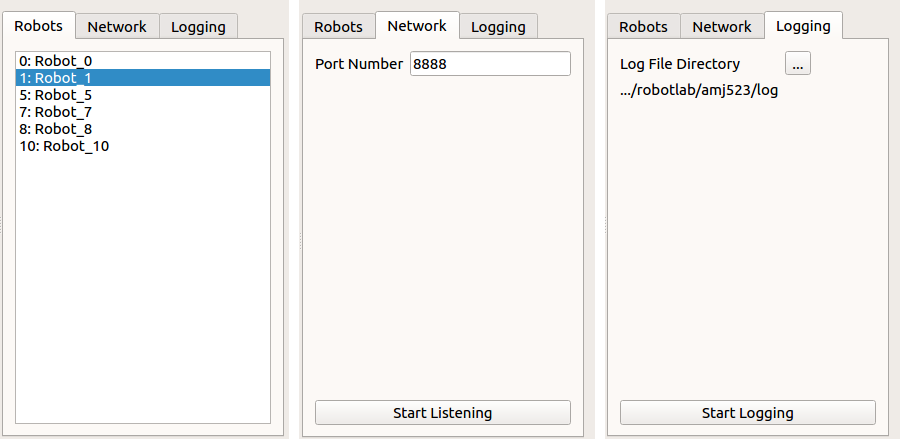
\includegraphics[width=1\textwidth]{Figures/RobotListPanel.png}}
 \decoRule
 \caption[Robot List Panel]{The robot list panel, showing all three tabs.}
 \label{fig:RobotListPanel}
\end{figure}

The data panel features five tabs. The first tab displays a simple text based console, which reports messages regarding the application itself, as well as any messages received from the robots in message packets. The messages are displayed sequentially, with the most recent message always being added as a new row at the bottom of the console. The second tab is the overview tab, which provides a summary of the selected robot's key data. The third tab is the state tab, which displays two lists of state information regarding the selected robot. The first lists all of the robot's known states, and the second lists recent state transitions, including the state before and after the transition, and the time at which the transition occurred. This should help the user to determine if a robot is moving through its states correctly, and check that it is not changing states out of order to too frequently. 

The fourth tab displays the selected robot's IR sensor data in the form of a bar graph. This includes two bars for each IR sensor, one for the active sensor reading and one for the background reading, with colour being used to differentiate between the two. The numerical values of both are also displayed below the bar, so that the user can ascertain the actual values if necessary. Finally the fifth tab displays the custom user data for the selected robot. This data is organised into a table showing the custom data keys in the first column, and the values for each respective key in the second column. All five tabs update their data in real time, in response to received packets. This means the user is kept up to date with the latest information immediately. Figure \ref{fig:DataPanel} shows the five data panel tabs.

\begin{figure}
 \centering
 \makebox[\textwidth][c]{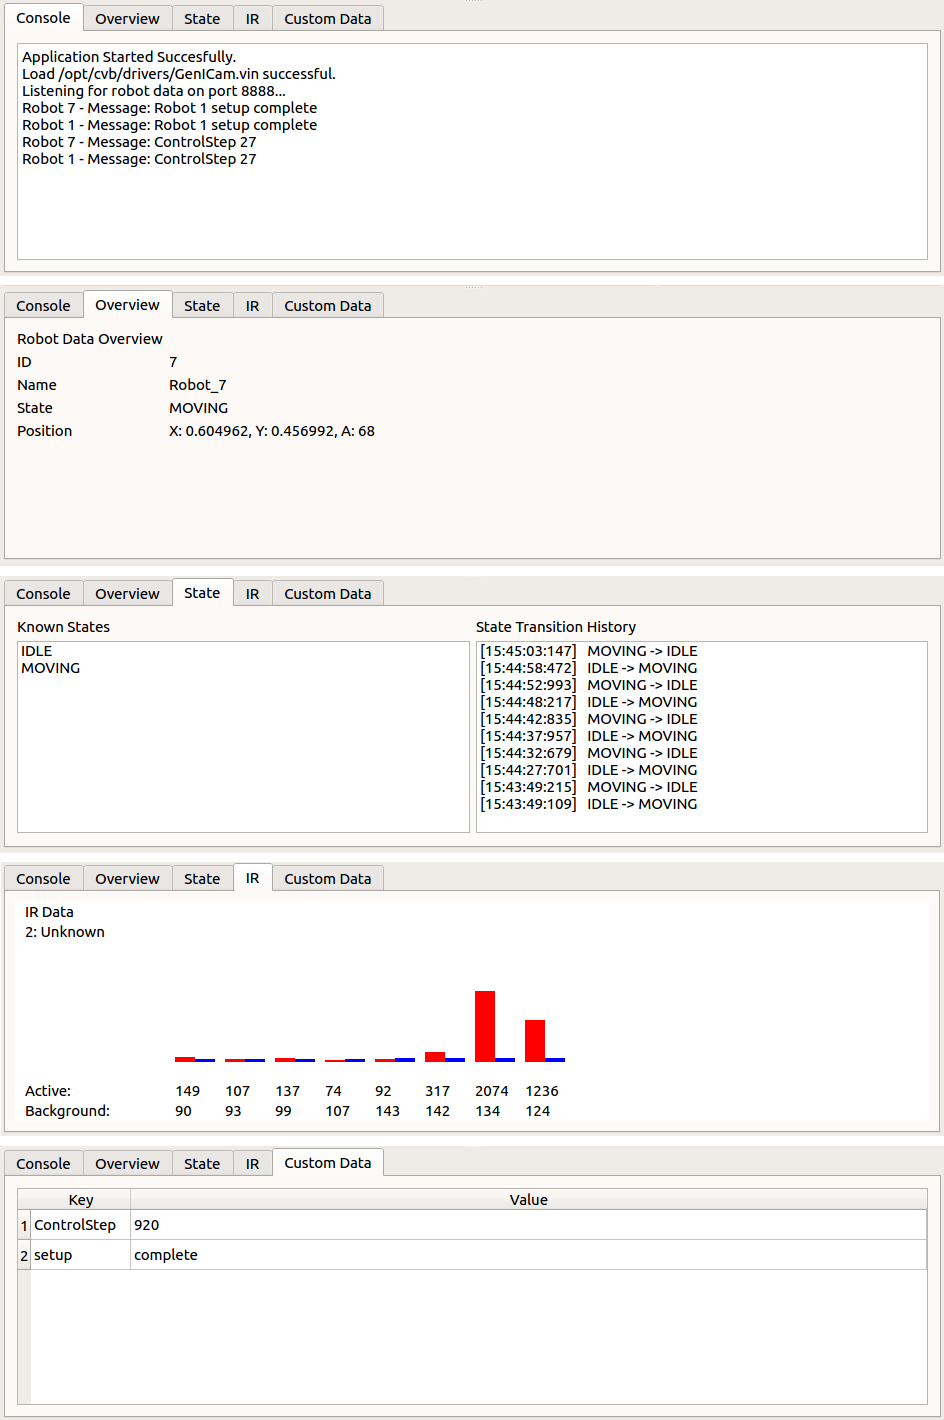
\includegraphics[width=1\textwidth]{Figures/DataPanel.png}}
 \decoRule
 \caption[Data Panel]{The data panel, showing all five tabs.}
 \label{fig:DataPanel}
\end{figure}

In addition to the main user interface, a number of extra `dialog' windows are used to provide the user with access to various settings. For each of the data visualisations which feature settings beyond a simple enable/disable , a dialog window class was implemented. The names of these classes take the form \textit{*SettingsDialog}, where \textit{*} is replaced by the visualisation type. The files containing definitions for these classes follow the same naming format, \textit{*settingsdialog.cpp / .h}. Dialog windows are a commonly used tool within applications programming. They act as pop-up windows which usually require the user to either confirm or cancel some action or change. In this case the dialog windows present controls for changing specific visualisation settings, and the user can then either apply their changes or cancel them using the standard accept/reject buttons at the bottom of the window.

%----------------------------------------------------------------------------------------

\section{Visualiser} \label{VisualiserImplementation}
The 'visualiser' is the name given to the custom user interface component that renders the augmented video feed. Implementing this component was key to satisfying the portion of the project aim related to augmented reality, and it forms one of the most visible elements of the system. The main visualiser component is defined in the \textit{Visualiser} class (\textit{visualiser.cpp / .h}), and a number of extra classes are used to define the associated settings and routines for visualising specific data types (\textit{VisConfig, VisID, VisName, VisState, VisPosition, VisDirection, VisProximity, VisPath and VisCustom}). Section \ref{VideoFeedAndTrackingSystem} describes the process of retrieving images from the camera and tracking the robots. The image data then arrives at the visualiser via a Qt slot function. At this stage the image is augmented based on the data in the data model, by iterating over the list of robots, and for each one iterating over the list of data visualisations, calling the render function for each. These render functions take the image and the current robot's data as arguments, and then add the relevant graphical representation to the image using the drawing functions within the OpenCV image processing library. This process is implemented following the design outlined in section \ref{VisualiserDesign}, and figure \ref{fig:VisualiserProcess}. 

\begin{figure}
	\centering
	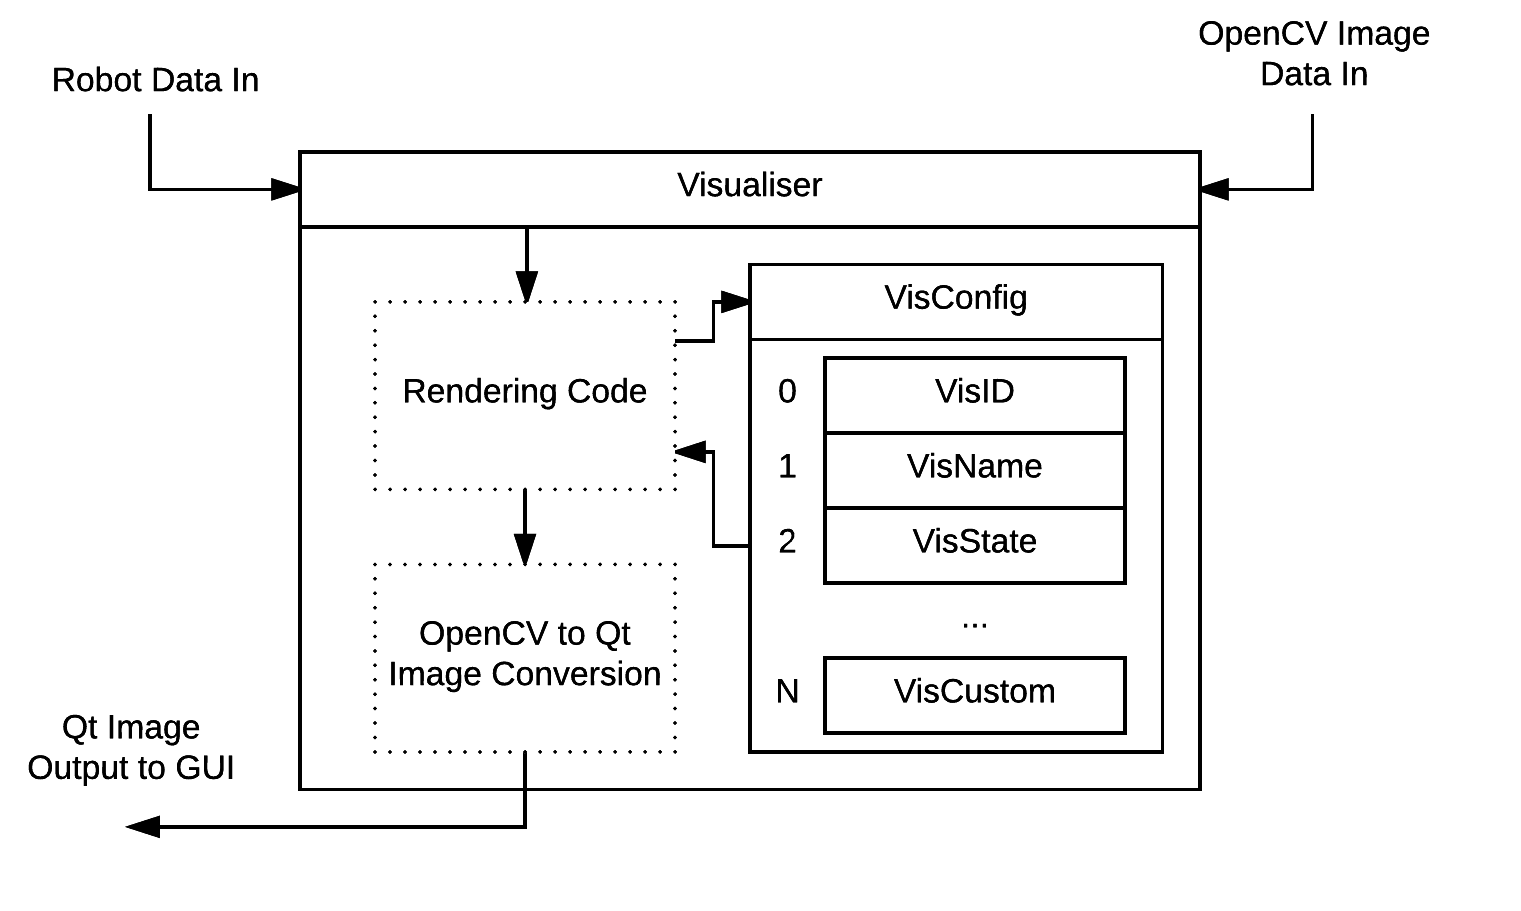
\includegraphics[scale=1]{Figures/VisualiserDiagram.png}
	\decoRule
	\caption[Visualiser Data Flow]{The path of data through the visualiser when generating each frame.}
	\label{fig:VisualiserDiagram}
\end{figure}

It was decided that an individual class would be implemented for each type of data visualisation. Each class derives from the abstract class \textit{VisElement}, which defines the general outline of a data visualisation class, and then each specific implementation defines how to generate the graphical overlay for that data type. The \textit{VisConfig} class stores a collection of all the \textit{VisElement}-derived objects, which can be iterated through to render each one. The use of an abstract class was necessary in order for the different visualisation element classes to be stored in the same collection. The overall aim of this implementation method was to make the visualisation process simpler to manage, and to follow object oriented practices, making it easier for new visualisation types to be added without modifying the underlying system. This also allows each data visualisation object to maintain its own settings, so that the visualiser component itself need not be aware of the details of the configuration of each data visualisation element. Instead each data visualisation element simply checks its own configuration when its render function is called. Figure \ref{fig:VisualiserDiagram} shows the flow of data through the visualiser when rendering a frame.

The rest of the code in the \textit{Visualiser} class relates to embedding the OpenCV image within a Qt UI widget, and tertiary functionality such as detecting clicks within the image frame, and retrieving the frame's size. The OpenCV to Qt image conversion is done by instantiating a QImage instance directly from the internal pixel data of the OpenCV image. This QImage is then drawn onto the widget. 

\subsection{Data Visualisations}
The visualiser supports a number of specific data visualisations:

\begin{enumerate}
 \item Highlighting robot position.
 \item Indicating robot 'orientation' by showing forward direction.
 \item Displaying the ID of a robot as text.
 \item Displaying the name of a robot as text.
 \item Displaying the current state of a robot as text.
 \item Displaying a graphical representation of a robot's IR sensor data.
 \item Displaying the recent path a robot has taken as a line behind the robot.
 \item Displaying a specific piece of custom data related to the robot as text.
\end{enumerate}

The designs for these visualisations described in section \ref{UserInterfaceDesign} and shown in figure \ref{fig:OverlayDesigns} were tested, and the most effective selected for the final implementation. Figure \ref{fig:Overlays} shows the implemented visualisations. Each row of figure \ref{fig:Overlays} is summarised as follows.

\begin{description}
\item [Row 1.] Shows all of the text-based visualisations individually, followed by the full set combined. The text based data is rendered adjacent to the robot, on the right hand side, where even relatively long strings will not overlap the robot's other visualisations. The exception to this is the ID number, which is rendered above and to the left, as this is unlikely to be long enough to cause overlapping issues.  

\item [Row 2.] Shows the robot position and orientation visualisations, alone and combined. Robot position is indicated using an outlined circle. This was chosen over the filled circle or square designs as it was the least intrusive on other elements of the image. Direction is indicated by a line, starting from the robot's centre and extending outwards in its forward direction. This was selected over the arrow based designs, as rendering the arrows at small enough sizes was not feasible.

\item [Row 3] Shows the two types of IR data visualisation. For the IR data visualisation, both designs were implemented, and the user can select which to use. The first renders a line for each of the sensors, extruding out from the centre of the robot at the angle of the respective sensor. The length varies inversely and non-linearly with the value of the sensor, in an attempt to approximate a proximity measurement. The second mode, referred to as the `heat map' mode, renders a number of small boxes around the robot, positioned to match the sensors. The colour and size of each box varies to indicate the sensor value. The choice to provide both was made because the line based visualisation is useful in certain scenarios when testing the response of individual sensors, but the box-based `heat map' visualisation provides a more immediately understandable indication of the sensor values.  

\item [Row 4.] Shows the path visualisation. The robot's recent path is visualised as a trail of line segments behind the robot. One of the original designs proposed a dotted line, but in the end this proved to be less visually clear than a solid line. The smoothness of the line was also considered in the design, but during implementation it became clear that the smoothness of the line was inherently related to the number of samples. A trade-off therefore had to be made between the smoothness and accuracy of the line, and its length. A setting was added to allow the user to vary the sampling interval for the line, thus allowing them to choose between a longer but less accurate and more jagged path, or a shorter but smoother and more accurate one.

\item [Row 5.] Finally row 5 shows two possible combinations of the visualisations. In the first the robot's ID, position and path are shown, as well as its IR data in heat map mode. In the second the robot's ID, name, state, position, direction and path are shown.
\end{description}

\vspace{2cm}
\begin{figure}[h]
	\centering
	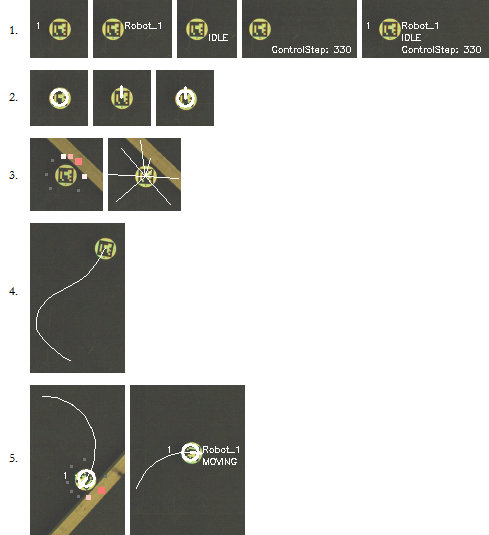
\includegraphics[scale=1]{Figures/Overlays.png}
	\decoRule
	\caption[Data Visualisations]{The different data visualisations as implemented.}
	\label{fig:Overlays}
\end{figure}

\clearpage
Each visualiser element can be enabled and disabled via the settings tab. Some of the visualisations have more complex settings, which can be accessed by double clicking the specific element in the visualisations list, also in the settings tab. For the majority of the visualisations the user has the option to set them to render only for the selected robot, or for all the robots. The IR data visualisation also has settings to switch between the proximity and heat map modes, and to set the angles of the sensors. The path visualisation has a setting for the sampling interval, as previously mentioned. Finally the custom data visualisation allows the user to input the key string for the data point they want displayed. Figure \ref{fig:VisualiserSettingsTab} shows the visualiser settings tab, as well as one of the dialog windows for accessing detailed visualisation settings. This dialog is showing the settings for the IR data visualisation.

\begin{figure}
 \centering
 \makebox[\textwidth][c]{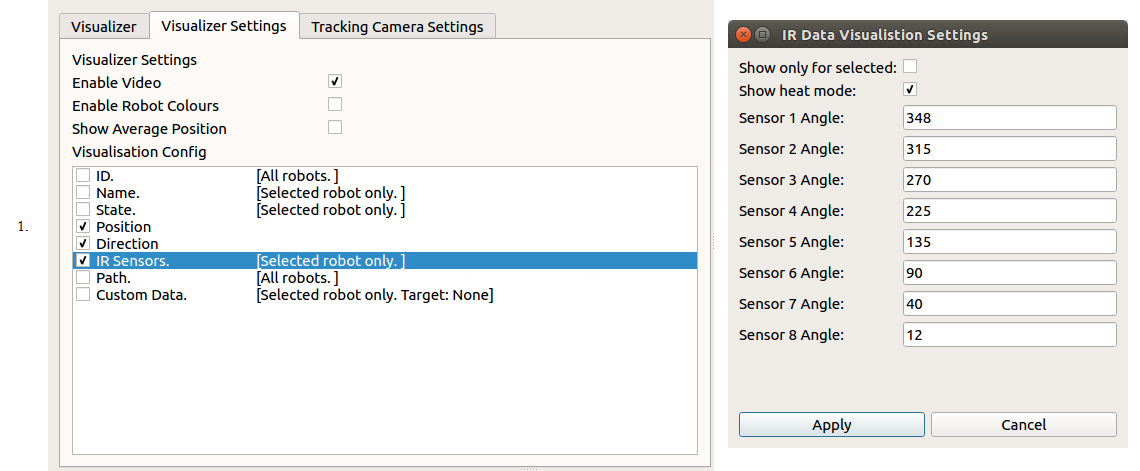
\includegraphics[width=1.2\textwidth]{Figures/VisualiserSettingsTab.png}}
 \decoRule
 \caption[Visualiser Settings Tab]{The visualiser settings tab, and one of the visualisation settings dialog windows.}
 \label{fig:VisualiserSettingsTab}
\end{figure}

%----------------------------------------------------------------------------------------

\section{Robot Side API} \label{RobotSide}
The robot side API is encapsulated by the \textit{DebugNetwork} class, defined in `\textit{debug\_network.cpp / .h}'. The contents of the \textit{DebugNetwork} class are described in appendix \ref{AppendixRobotAPI}, table \ref{tab:RobotAPI}.

In order to utilise this API a user should modify their robot controller code to include the \textit{debug\_network.h} header file, call the \textit{init} function at start-up time, and then call the various data reporting functions whenever necessary. The user is therefore in charge of how frequently data is transmitted, and can decide whether to simply send updates to the application when the robot's data changes, or to transmit a fixed quantity of data every control step.

It was potentially possible for the API to handle all data reporting in the background, without requiring the user to specify when to transmit data in the controller code, however this approach was not taken for a number of reasons. Firstly it limits the control and flexibility available to the user. Each swarm system is different, and may have different requirements, hence the API should allow the developer to make decisions regarding data reporting which are right for their specific case. It would also limit the portability of the API, as a more automatic system would likely need to hook into the lower level robot drivers, meaning much greater changes would be necessary to port the code to a different robot. Furthermore by allowing the user to have complete control over when and how frequently data is transmitted they are able to manage the amount of traffic they are putting on their network, potentially mitigating congestion issues with very large swarms. Finally allowing users to control the moments within the code when data is reported to the debugging system was deemed to be a more intuitive system, especially as many developers are already familiar with the concept of using `print' statements within code to display debugging messages in a console.

%----------------------------------------------------------------------------------------

\section{Summary}
This chapter began with a discussion of the choice of application programming framework for implementing this application, establishing the reasons for choosing the \textit{Qt} framework. Following this key decision the implementation of the system is then described, including the overall structure of the system, and details of the functioning of each key component. The implementation of code for use on the robots is also discussed. This chapter summarises the work completed for the implementation portion of the project plan, outlined in chapter \ref{ChapterPlan}.